\documentclass{article}
\usepackage[margin=1in]{geometry}
\usepackage{amsmath}
\usepackage{graphicx}
\usepackage{hyperref}
\usepackage{url}
\usepackage{fancyvrb}
\usepackage{listings}

\begin{document}
\title{Zumy Tutorial}
\author{James Lam Yi}
\date{\today}
\maketitle
This document provides an introduction to Zumy robotic platform and a tutorial of controlling this platform for navigation in a ROS environment. We provide examples for using \verb=RQT robot steering=\footnote{\url{http://wiki.ros.org/rqt_robot_steering}} and \verb=turtlesim=\footnote{\url{http://wiki.ros.org/turtlesim}} package in ROS for driving Zumy. 

\section{Introduction}
\begin{figure}[h]
\centering
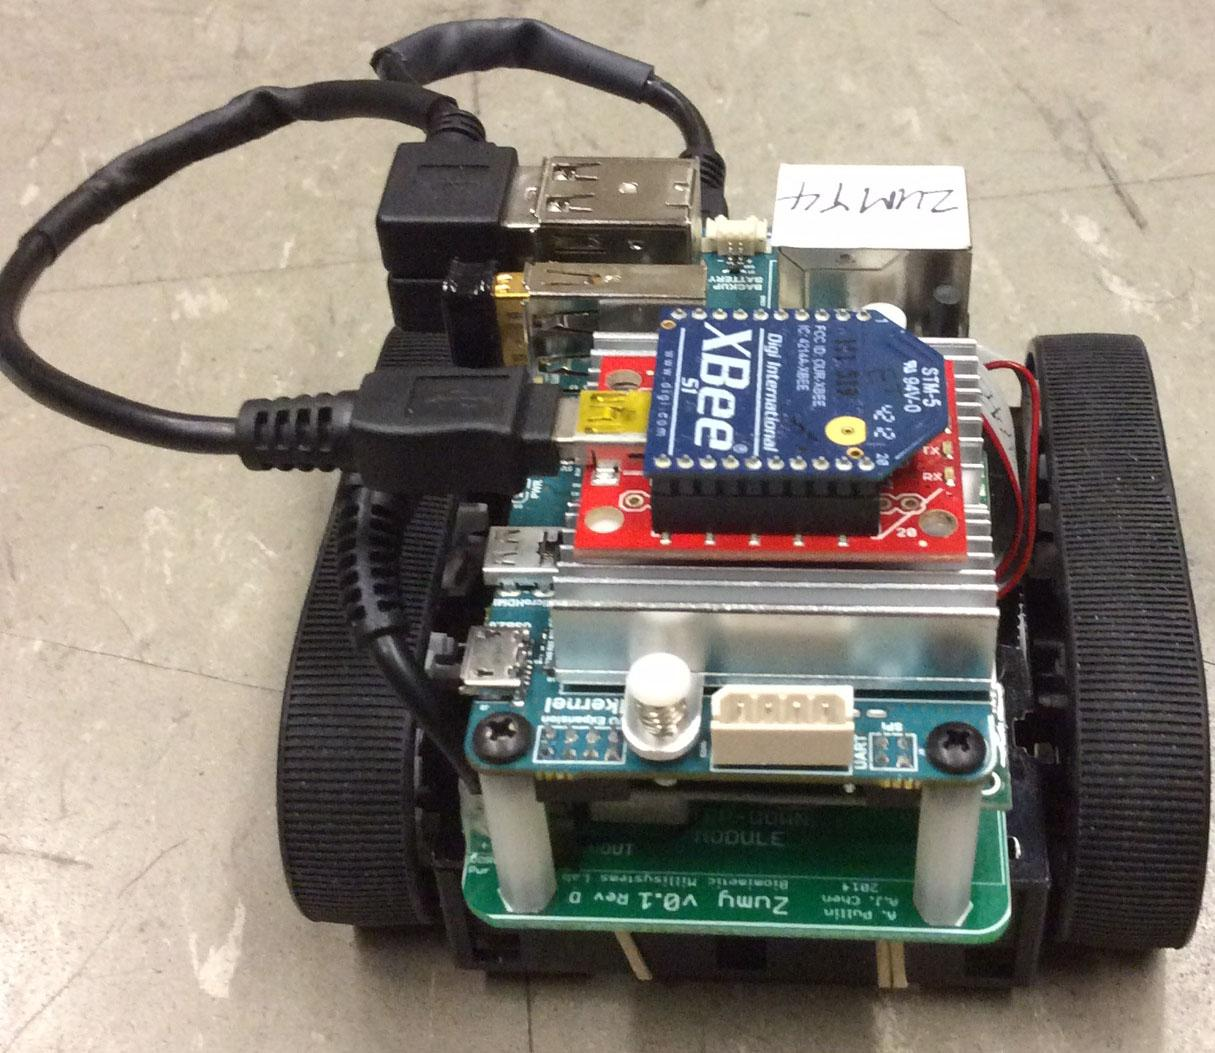
\includegraphics[width=0.6\textwidth]{img/zumy.jpg}
\caption{Zumy Robotic platform}
\label{fig:zumy}
\end{figure}
The Zumy Robotic platform is being developed and used in Fearing Biomimetic Millisystems Laboratory as a Linux-Based mobile platform for cooperative exploration and mapping applications. The Zumy robot is an ODROID-U3 embedded Linux Computer connected to an mbed LPC1768 board, sitting on top of differential drive tank chassis. It is shown in Figure \ref{fig:zumy}. The ODROID runs Ubuntu 14.04, and ROS Indigo base libraries are installed. The communication between Zumy and the host is based on ROS enviroment.

\section{Navigation}
\subsection{ROS host setup}
In order to enable communication via ROS, ROS host name and master should be set up. First, check out the host name with

\begin{Verbatim}[frame=single]
vim /etc/hostname
\end{Verbatim}

Then set up ROS host name and master by editing this file

\begin{Verbatim}[frame=single]
sudo gedit ~/.bashrc
\end{Verbatim}

Insert these two lines to the end of this file

\begin{Verbatim}[frame=single]
export ROS_HOSTNAME="your host name".local
export ROS_MASTER_URI=http://"your host name".local:11311
\end{Verbatim}

Save and exit, and then source the file

\begin{Verbatim}[frame=single]
source ~/.bashrc
\end{Verbatim}

If these steps has been done in previous tutorials, skip this section.

If ROS host name and master are not set up before launching connections with Zumy, the following errors may show up

\begin{Verbatim}[frame=single]
gaierror: [Errno -2] Name or service not known
\end{Verbatim}

\begin{Verbatim}[frame=single]
connection refused
\end{Verbatim}

\subsection{Zumy setup}
Zumy is set to examine the local network connection with the ROS host when it boots. If it detects no connection with the ROS host, it attemps to reconnect at most 3 times. To enable this function, at first, open this file \verb=on the Zumy= you have (with SSH or Odroid USB-UART Module Kit)
\begin{Verbatim}[frame=single]
vim /home/zumy/network_test.sh
\end{Verbatim}
And edit this line with the ROS host name you obtain from last section
\begin{Verbatim}[frame=single]
host="your host name"
\end{Verbatim}
Finally, restart Zumy

\subsection{SSH key setup}
SSH with a passphrase will prompt the user for a password when connecting to the remote host. To drive Zumy, however, the host needs to establish SSH connections without passing a passphrase. The SSH key needs to be set up \verb=only once= to establish the connection. The guide below shows the steps to set up this key:

\begin{enumerate}
\item Check out the host name of the Zumy you have. There is a number written on top of ethernet port of each Zumy. For a Zumy labeled number 'x', its host name is set to 'zumyx'. For example, the host name of a Zumy labeled '3' is 'zumy3'.
\item Generate the public private key on the host
\begin{Verbatim}[frame=single]
ssh-keygen -t rsa -f ~/.ssh/id_rsa
\end{Verbatim}
\item Copy the public key to the Zumy you will connect to
\begin{Verbatim}[frame=single]
scp ~/.ssh/id_rsa.pub zumy@zumyx.local:~/.ssh/id_rsa.pub
\end{Verbatim}
Modify "zumyx" above to the host name of your Zumy. This command should prompt you a password, and the password for Zumy is "zumy".
\item Shell into Zumy
\begin{Verbatim}[frame=single]
ssh zumy@zumyx.local
\end{Verbatim}
Again, "zumyx" should be the host name of your Zumy, and the same password mentioned from last step is required.
\item Authorize the key by adding it to the list of authorized keys
\begin{Verbatim}[frame=single]
cat ~/.ssh/id_rsa.pub >> ~/.ssh/authorized_keys
\end{Verbatim}
\item Log out of the current shell
\begin{Verbatim}[frame=single]
exit
\end{Verbatim}
\item Test that you can log in with no password
\begin{Verbatim}[frame=single]
ssh zumy@zumyx.local
\end{Verbatim}
If this prompts for a password, log in your Zumy with
\begin{Verbatim}[frame=single]
ssh zumy@zumyx.local
\end{Verbatim}
Delete the saved SSH key with
\begin{Verbatim}[frame=single]
ssh-keygen -R "host name of your Zumy"
\end{Verbatim}
And repeat the above steps again.
\item Add SSH key of Zumy into your host known hosts 
\begin{Verbatim}[frame=single]
ssh-keyscan zumyx.local >> .ssh/known_hosts
\end{Verbatim}
If you succeeded, you will see the output is like
\begin{Verbatim}[frame=single]
# zumyx.local SSH-2.0-OpenSSH_6.6p1 Ubuntu-2ubuntu1
\end{Verbatim}
Output may not be the same due to different SSH versions and operating systems. If not, remove SSH key on the host with
\begin{Verbatim}[frame=single]
ssh-keygen -R "host name of your Zumy"
\end{Verbatim}
And repeat this step again.
\end{enumerate}


\subsection{Odroid machine}
\verb=Odroid machine=\footnote{\url{http://github.com/jlamyi/odroid_machine}} is a ROS package developed in Fearing Biomimetic Millisystem Laboratory for establishing communication between Zumy and the host. It indicates if a Zumy is connected to the host, and awake Zumy to wait for commands in ROS environment. Following steps are setup and tests for this package:

\begin{enumerate}
\item Install dependencies
\begin{Verbatim}[frame=single]
sudo apt-get install python-nmap ros-indigo-zeroconf-avahi-suite
\end{Verbatim}
Python-subprocess is a build-in module in python. If it cannot be found, re-install python.
\item Download the package to the \verb=src= directory of a ROS workspace with
\begin{Verbatim}[frame=single]
git clone https://github.com/jlamyi/odroid_machine.git
\end{Verbatim}
\item Run \verb=catkin_make= from the workspace (this may take a while).
\item Turn on Zumy, and test the local network connection with
\begin{Verbatim}[frame=single]
ping "host name of your Zumy".local
\end{Verbatim} 
If packages are received from Zumy, the local network connection is good (It takes a while for Zumy to connect to the network after it is turned on). Otherwise, restart Zumy, and repeat this step.
\item Start ROS connection with Zumy
\begin{Verbatim}[frame=single]
roslaunch odroid_machine remote_zumy.launch mname:="host name of your Zumy"
\end{Verbatim}
If the connection is setup successfully, Zumy's wheels will move a little bit, and terminal ouput should be like
\begin{Verbatim}[frame=single]
... done launching nodes
\end{Verbatim}
If it fails, restart Zumy and repeat from last step. A good ROS connection must be set up before sending commands to Zumy in the following sections. 
\end{enumerate}
Also, once you succeed, \verb=rqt_graph=\footnote{\url{http://wiki.ros.org/rqt_graph}} should display Figure \ref{fig:rqt_graph}, which shows that Zumy is subscribing topic \verb=/cmd_vel= under the namespace of its host name. 
\begin{figure}[h]
\centering

\includegraphics[width=0.6\textwidth]{img/rosgraph.png}
\caption{RQT Graph using Odroid machine}
\label{fig:rqt_graph}
\end{figure}

\subsection{RQT robot steering}

One way to drive Zumy is to use \verb=RQT robot steering=, which provides a GUI plugin for steering a robot using Twist messages. Once Zumy establishes a good ROS connection with the host, run \verb=RQT robot steering= with

\begin{Verbatim}[frame=single]
rosrun rqt_robot_steering rqt_robot_steering
\end{Verbatim} 
After robot steering GUI starts, modify pubilish topic name to 

\begin{Verbatim}[frame=single]
/"host name of your Zumy"/cmd_vel
\end{Verbatim}

\begin{figure}[h]
\centering
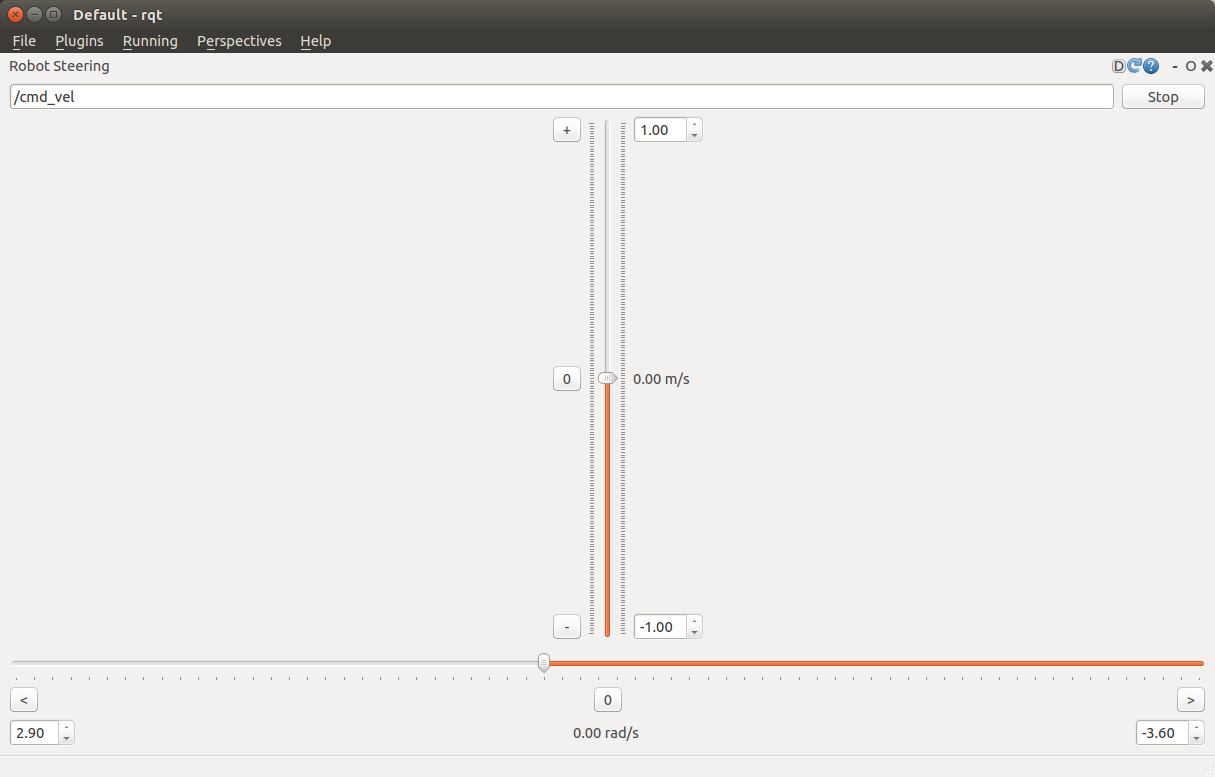
\includegraphics[width=1\textwidth]{img/rqt_robot_steering.png}
\caption{RQT robot steering plugin GUI}
\label{fig:robot_steering}
\end{figure}
After modification, pulling the bar on the top up and down allows you to move Zumy forward and backward, and pulling the bar on the bottom left and right allows you to turn Zumy left and right.


\subsection{Turtlesim}
The other way to drive Zumy is to use \verb=turtlesim=, which allows users to input navigation commands using a keyboard. \verb=zumy_teleop=\footnote{\url{https://github.com/jlamyi/zumy_teleop}}, developed in Fearing Biomimetic Millisystem Laboratory, is a ROS wrapper package based on \verb=turtlesim= for bridging \verb=turtlesim= and Zumy. This package can be downloaded with

\begin{Verbatim}[frame=single]
git clone https://github.com/jlamyi/zumy_teleop.git
\end{Verbatim}
When the download is finished, compile the package from the workspace by running \verb=catkin_make=. Once Zumy establishes a good ROS connection with the host (Section \verb=Odroid machine= is required to be completed), launch \verb=zumy_teleop= with

\begin{Verbatim}[frame=single]
roslaunch zumy_teleop zumy_teleop.launch mname:="host name of your Zumy"
\end{Verbatim}

Now you can use the arrow keys of the keyboard to drive Zumy around. If you cannot drive Zumy with keyboard, make sure the connection bewteen the host and Zumy is good. If the connection is good, restart all the ROS nodes running on the host.

\end{document}
